\documentclass{article}
\usepackage[utf8]{inputenc}
\usepackage[greek, brazil]{babel}
\usepackage[left=1cm, right=1.5cm, top=5cm, bottom=5cm]{geometry}
\usepackage{amsmath}
\usepackage{amsfonts}
\usepackage{amssymb}
\usepackage{makeidx}
\usepackage{graphicx}
\usepackage{hyperref}
\usepackage[usenames,dvipsnames]{xcolor}
\renewcommand{\thefootnote}{\alph{footnote}}
\setlength{\parskip}{\baselineskip}
\setlength{\parindent}{0pt}
\hypersetup {
  colorlinks,
  citecolor = NavyBlue,
  filecolor = NavyBlue,
  linkcolor = NavyBlue,
  urlcolor = NavyBlue
}
\author{Sadron}
\title{Laboratório 7 - Tratamento de Exceção\\ \small{considere a motivação 
alheia, questione tudo.}}
\begin{document}
\maketitle

\section{Fibonacci}

Seta \$s0 com o endereço base dos registradores de \textbf{MMIO}.

\begin{verbatim}
move $t2, $zero
lui $s0, 0xffff
\end{verbatim}

Habilite as interrupções para entradas de teclado.

\begin{verbatim}
lw $t2, 0($s0)
ori $t2, $t2, 0x2
sw $t2, 0($s0)
\end{verbatim}

\pagebreak
{\bfseries Pergunta: em que instrução ocorre overflow na série de fibonacci em 
linguagem de máquina, experimente tratar o processo no momento em que você 
capta se é overflow ou não, para testar você mesmo, eu posso estar errado.?}

\begin{center}
Pista: \textbf{return} \verb|fib(n-1)| {\Huge\textbf{\color{Red} +}} 
\verb|fib(n-2)|
\end{center}

\begin{figure}[ht!]
\centering
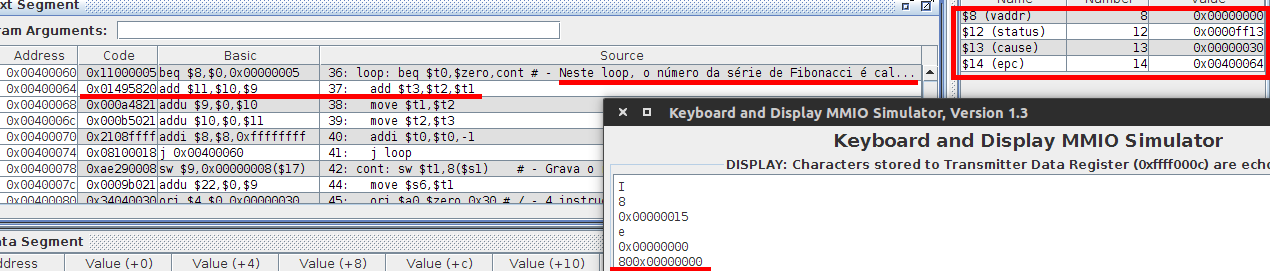
\includegraphics[scale=0.4]{overflow}
\end{figure}

\section{Tratador de Exceções}

Etapa 1 - Salvamento de contexto: Os registradores usados pelo tratador são
preservados, o que não pode ser feito usando a pilha.

\begin{verbatim}
lui $k0,0x9000
sw $ra,0($k0)
sw $at,4($k0)
sw $t0,8($k0)
sw $t1,12($k0)
\end{verbatim}

Etapa 2 - Decodificação do registrador de causa: O objetivo é descobrir a causa
da exceção para realizar a ação apropriada (por exemplo, se for uma interrupção,
fazer a leitura e o processamento do valor digitado).

\begin{verbatim}
mfc0 $k1, $13
srl $t0, $k1, 0x2
andi $t0, $t0, 0xf
\end{verbatim}

Etapa 3 – Tratamento de interrupção: Leitura da posição de memória
\verb|0xFFFF0004| e processamento do valor digitado. Isso é feito chamando um
procedimento \verb|lechar|.

\begin{verbatim}
bne $t0, $zero, _continua
jal lechar
j done
\end{verbatim}

Etapa 4 - Tratamento de \verb|overflow|: O cálculo de um número da série de
Fibonacci pode resultar em \verb|overflow| em função do índice digitado. Nesse
caso, é preciso tratar o \verb|overflow|, o que deve ser feito imprimindo um “I”
no \verb|display| do usuário e reiniciando o programa.

\begin{verbatim}
add $t1, $zero, 12
bne $t0, $t1, done

la $t1, main
mtc0 $t1, $14
\end{verbatim}

Etapa 5 - Preparação do sistema para novas exceções: Consiste na atualização dos
registradores Cause e Status para habilitar o tratamento de novas exceções que
vierem a ser detectadas.

\begin{verbatim}
mfc0 $k0, $14
addiu $k0, $k0, 4
mtc0 $k0, $14
mtc0 $0, $13
mfc0 $k0, $12
ori $k0, $k0, 0x1
mtc0 $k0, $12
\end{verbatim}

Etapa 6 - Restauração de contexto: Recuperação dos valores de registradores
preservados.

\begin{verbatim}
lui $k0,0x9000
lw $ra,0($k0)
lw $at,4($k0)
lw $t0,8($k0)
lw $t1,12($k0)
\end{verbatim}

Etapa 7 - Retorno ao fluxo normal de execução ou ao início do programa: No caso
da exceção gerada pelo uso do teclado (interrupção), voltar à execução da
instrução que deveria ter sido executada. No caso de \verb|overflow|, reiniciar
o programa.

\begin{verbatim}
eret
\end{verbatim}

\end{document}
